%%%%%%%%%%%%%%%%%%%%%%%%%%%%%%%%%%%%%%%%%
%
% (c) 2019 by Jennifer Laaser
%
% This work is licensed under the Creative Commons Attribution-NonCommercial-ShareAlike 4.0 International License. To view a copy of this license, visit http://creativecommons.org/licenses/by-nc-sa/4.0/ or send a letter to Creative Commons, PO Box 1866, Mountain View, CA 94042, USA.
%
% The current source for these materials is accessible on Github: https://github.com/jlaaser/pogil-polymers
%
%%%%%%%%%%%%%%%%%%%%%%%%%%%%%%%%%%%%%%%%%

\renewcommand{\figpath}{content/polymphys/solution-thermo/flory-huggins/figs}

\begin{activity}[Regular Solutions \& Flory-Huggins Theory]

\begin{instructornotes}

	This activity introduces students to key concepts related to polymer solutions, including ideal mixing, regular solution theory, and Flory-Huggins theory.
	
	After completing this activity, students will be able to:
			\begin{enumerate}
				\item ...
			\end{enumerate}
	This activity will prepare students for follow-up activities on phase diagrams for polymer solutions.
			
	\subsection*{Activity summary:}
	\begin{itemize}
		\item \textbf{Activity type:} Learning Cycle
		\item \textbf{Content goals:} Ideal mixing, regular solution theory, and Flory-Huggins theory
		\item \textbf{Process goals:} %https://pogil.org/uploads/attachments/cj54b5yts006cklx4hh758htf-process-skills-official-pogil-list-2015-original.pdf
			written communication, critical thinking, information processing
		\item \textbf{Duration:} TBD
		\item \textbf{Instructor preparation required:} none beyond knowledge of relevant content
		\item \textbf{Related textbook chapters:}
			\begin{itemize}
				\item \emph{Polymer Chemistry} (Hiemenz \& Lodge): sections 7.1-7.3
		\end{itemize}
	\end{itemize}

\end{instructornotes}

	%\textbf{Focus question:} Put a central question for the students to consider through this exercise here.

\begin{model}[Ideal Mixtures: Entropy of Mixing]

A simple model for mixing of two small-molecule liquids is shown below.  In this model, each molecule is shown as a circle, and we place them in a grid where each molecule takes up exactly one ``space'' in the grid.

Initially, the molecules of each type are isolated in their own containers:

\centerline{\includegraphics[width=0.6\textwidth]{\figpath/model1-initial}}

After combining the two containers, the molecules mix together:

\centerline{\includegraphics[width=0.3\textwidth]{\figpath/model1-mixed}}

The critical elements of this model are that
\begin{enumerate}[itemsep=0pt,topsep=-6pt]
	\item the number of molecules of each type does not change,
	\item the molecules each take up exactly the same volume (here, one square on the grid),
	\item the total volume after mixing is the sum of the two initial volumes, and
	\item the mixing is entirely random.
\end{enumerate}

\end{model}

\vspace{0.05in}
\begin{ctqs}

	\question Consider a simple, specific case of this model, as shown below:

\centerline{\includegraphics[width=0.7\textwidth]{\figpath/model1-simplified}}

		Here, $m_1=2$ (there are two molecules of type 1, shown as open circles) and $m_2=2$ (there are two molecules of type 2, shown as filled circles).
	
		\begin{enumerate}
			\item How many different ways can you distribute the two molecules of type 1 in their initial box, assuming the molecules are indistinguishable (you can't tell them apart)?  Sketch the possible configurations below.  Note that you may not need to use all of the boxes; cross off any you don't need.
			
				\begin{solution}
					\studentdisplay{

\centerline{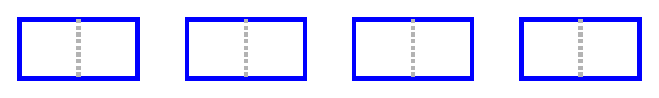
\includegraphics[width=0.6\textwidth]{\figpath/model1-2blank}}

						\vspace{0.1in}
						\centerline{Number of configurations ($\Omega_1$) = $\rule{1cm}{0.15mm}$}
					}
					\instructordisplay{

\centerline{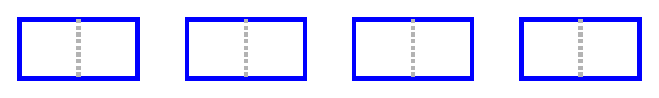
\includegraphics[width=0.6\textwidth]{\figpath/model1-2blank}}

						\vspace{0.1in}
						\centerline{Number of configurations ($\Omega_1$) = $\rule{1cm}{0.15mm}$}
					}
				\end{solution}
		
			\item How many different ways can you distribute the two molecules of type 2 in their initial box, assuming the molecules are indistinguishable (you can't tell them apart)?  Sketch the possible configurations below. Again, you may not need to use all of the boxes.
			
				\begin{solution}
					\studentdisplay{

\centerline{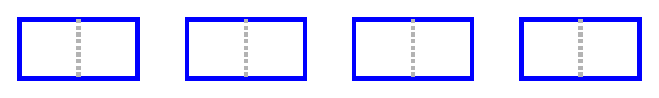
\includegraphics[width=0.6\textwidth]{\figpath/model1-2blank}}

						\vspace{0.1in}
						\centerline{Number of configurations ($\Omega_2$) = $\rule{1cm}{0.15mm}$}
					}
					\instructordisplay{

\centerline{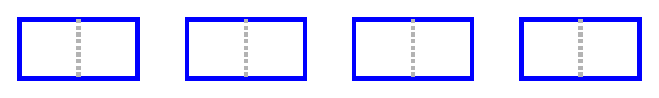
\includegraphics[width=0.6\textwidth]{\figpath/model1-2blank}}

						\vspace{0.1in}
						\centerline{Number of configurations ($\Omega_2$) = $\rule{1cm}{0.15mm}$}
					}
				\end{solution}
			
			\item How many different ways can you distribute the four molecules in the final mixture, assuming that you can't distinguish molecules of the same type from each other?  Again, you may not need to use all of the boxes.
			
				\begin{solution}
					\studentdisplay{

\centerline{\includegraphics[width=0.6\textwidth]{\figpath/model1-4blank}}

						\vspace{0.1in}
						\centerline{Number of configurations ($\Omega_{mixed}$) = $\rule{1cm}{0.15mm}$}
					}
					\instructordisplay{

\centerline{\includegraphics[width=0.6\textwidth]{\figpath/model1-4blank}}

						\vspace{0.1in}
						\centerline{Number of configurations ($\Omega_{mixed}$) = $\rule{1cm}{0.15mm}$}
					}
				\end{solution}
		\end{enumerate}
		
	\question Recall that if $\Omega$ is the number of ways that the molecules in the system can be arranged, then the entropy of that system is given by
		\begin{equation*}
			S = k \ln \Omega
		\end{equation*} 
		where $k$ is the Boltzmann constant.  Using this relationship, and your answers from question 1, calculate
			
		\begin{enumerate}
			\item the entropy of the initial state ($S_{initial} = S_1 + S_2$, where $S_1 = k\ln \Omega_1$ and $S_2 = k \ln \Omega_2$):
				\begin{solution}[1.25in]
				\end{solution}
			\item the entropy of the final (mixed) state, $S_{mixed}$):
				\begin{solution}[1in]
				\end{solution}
			\item the change in entropy upon mixing ($\Delta S_{mix} = S_{mixed} - S_{initial}$): 
				\begin{solution}[1in]
				\end{solution}
		\end{enumerate}
		
\end{ctqs}

\begin{infobox}
	Mathematically, the number of ways to fill $N$ boxes with $n$ indistinguishable molecules of type 1 and $N-n$ indistinguishable molecules of type 2 is
	\begin{equation*}
		\Omega = {N \choose n} = \frac{N!}{n!(N-n)!}
	\end{equation*}
	where $n! = n\cdot(n-1)\cdot(n-2)\cdot\dots\cdot 2 \cdot 1$.
	
	Note that by definition, $0!=1$.
\end{infobox}

\vspace{0.05in}
\begin{ctqs}
		
		\question For the initial state of the system shown in Model 1,
			\begin{enumerate}
				\item What are $N$ and $n$ for \emph{just} the type-1 molecules in the initial state?
				
					\begin{solution}[0.75in]
						\begin{align*}
							N = m_1 && \text{and} && n = m_1
						\end{align*}
					\end{solution}
					
				\item Using the mathematical expression given above, calculate $\Omega_1$, the number of configurations accessible to the type-1 molecules in the initial state.
				
					\begin{solution}[1.5in]
						\begin{equation*}
							\Omega_1 = {m_1 \choose m_1} = \frac{m_1!}{m_1! 0!} = 1
						\end{equation*}
					\end{solution}
				
				\item Similarly, what is $\Omega_2$, the number of configurations accessible to the type-2 molecules in the initial state?
				
					\begin{solution}[1in]
						$\Omega_2$ should also equal 1.
					\end{solution}
					
				\item What is the total entropy of the initial state?
					
					\begin{solution}[1in]
						\begin{equation*}
						S_{initial} = k \ln \Omega_1 + k \ln \Omega 2 = k \ln 1 + k \ln 1 = 0
						\end{equation*}
					\end{solution}
			\end{enumerate}
		
		\question For the final (mixed) state of the system shown in Model 1, 
			\begin{enumerate}
				\item What are $N$ and $n$ for the final (mixed) state?
				
					\begin{solution}[0.75in]
						\begin{align*}
							N = m_1+m_2=m && \text{and} && n = m_1
						\end{align*}
					\end{solution}
					
				\item Write an expression for the number of configurations possible for the final (mixed) state in terms of $m_1$ and $m_2$.
				
					\begin{solution}[1in]
						\begin{equation*}
							\Omega_{mixed} = {(m_1+m_2) \choose m_1} = \frac{(m_1+m_2)!}{m_1! m_2!} = \frac{m!}{m_1! m_2!}
						\end{equation*}
					\end{solution}
					
				\item What is the entropy of the final (mixed) state?
				
					\begin{solution}[1in]
						\begin{align*}
							S_{mixed} &= k \ln \Omega_{mixed}\\
							&= \ln m! - \ln m_1! - \ln m_2!
						\end{align*}
					\end{solution}
				
				
			\end{enumerate}
		\question What is the entropy of mixing, $\Delta S_{mix} = S_{mixed} - S_{initial}$, for the system shown in Model 1?
				
					\begin{solution}[1in]
						\begin{align*}
							\Delta S_{mix} &= S_{mixed} - S_{initial}\\
							 &= \ln m! - \ln m_1! - \ln m_2! - 0 \\
							 &= \ln m! - \ln m_1! - \ln m_2!
						\end{align*}
					\end{solution}
\end{ctqs}

\begin{infobox}
	Logarithms of factorials can be approximated using Stirling's approximation,
	\begin{equation*}
		\ln N! \approx N \ln N - N \label{eqn:stirling}
	\end{equation*}
	Using this approximation, it is possible (after some algebra) to rewrite your expression for $\Delta S_{mix}$ as
	\begin{equation*}
		\Delta S_{mix} = -k\left(m_1 \ln\left(\frac{m_1}{m}\right) + m_2 \ln\left(\frac{m_2}{m}\right) \right)
	\end{equation*}
\end{infobox}

\begin{ctqs}
	\question As written, is $\Delta S_{mix}$ an \emph{extensive} property (which depends on the total number of molecules in the system) or an \emph{intensive} property (which does not depend on the total number of molecules present)?  Briefly explain your answer in 1-2 complete sentences.
	
		\begin{solution}[1.5in]
		\end{solution}
	
	\question Usually, it is most convenient to divide by the total number of molecules, which leaves us with an intensive expression for the entropy,
		\begin{equation*}
			\Delta S_{mix}^{(int)} = \frac{1}{m} \Delta S_{mix}
		\end{equation*}
		Write an expression for $\Delta S_{mix}^{(int)}$ in terms of $m_1$, $m_2$, and $m$.
		
			\begin{solution}[1in]
			
				\begin{equation*}
					\Delta S_{mix}^{(int)} = -k\left(\frac{m_1}{m} \ln\left(\frac{m_1}{m}\right) + \frac{m_2}{m} \ln\left(\frac{m_2}{m}\right) \right)
				\end{equation*}
			\end{solution}
		
	\question We also often prefer to work in terms of \emph{mole fractions} rather than numbers of molecules. \label{ctq:Smixed}
	
		Rewrite your expression for $\Delta S_{mix}^{(int)}$ in terms of the mole fractions
		\begin{align*}
			x_1 = \frac{m_1}{m_1 + m_2} = \frac{m_1}{m} && \text{and} && x_2 = \frac{m_2}{m_1+m_2} = \frac{m_2}{m}
		\end{align*}
		
			\begin{solution}[1in]
			
				\begin{equation*}
					\Delta S_{mix}^{(int)} = -k\left(x_1 \ln x_1 + x_2 \ln x_2 \right)
				\end{equation*}
			\end{solution}
		
	\question The mole fractions, $x_1$ and $x_2$, must both be between 0 and 1.  In this case,
		\begin{enumerate}
			\item Will $\ln x_1$ (and $\ln x_2$) be positive or negative?
	
				\begin{solution}[1in]
				\end{solution}
				
			\item Will $\Delta S_{mix}^{(int)}$ be positive or negative? \label{ctq:Spositive}
	
				\begin{solution}[1in]
				\end{solution}
				
		\end{enumerate}
		
	\question Explain, in 1-2 complete sentences, why we say that ideal mixing is an \emph{entropy-driven} process.
	
		\begin{solution}[1.5in]
		\end{solution}
		
\end{ctqs}
	

\begin{model}[Real Mixtures: Enthalpy of Mixing]

In an \emph{ideal} mixture, the molecules do not interact with each other, and entropy is the only thermodynamic consideration that affects mixing.
In real mixtures, however, molecules do interact with each other, and we must take those interactions into account when determining whether mixing is favorable or unfavorable.

To incorporate the energetics of intermolecular interactions into our model, we must make two key assumptions:
\begin{enumerate}
	\item First, we assume that molecules interact only with their immediate neighbors, and that each interaction involves only two molecules.  The interaction energies between different types of pairs are as follows:

\centerline{\includegraphics[width=0.5\textwidth]{\figpath/model2-interactions}}
	
	\item Second, we assume that each molecule has some number of neighbors, $z$, which we refer to as the ``coordination number''.  For example, the central molecule shown below has 4 nearest neighbors, so its coordination number is 4:

\centerline{\includegraphics[width=0.18\textwidth]{\figpath/model2-coordnum}}

		%Note that when drawing the molecules on a square lattice like this, we do not count molecules positioned diagonally from each other as being ``neighbors''.

\end{enumerate}

\end{model}

\begin{ctqs}

	\question In the initial state (before mixing), 
		\begin{itemize}[itemsep=0pt,topsep=3pt]
			\item there are $m_1$ molecules of type 1 that each have $z$ neighbors of type 1, for a total interaction energy of $H_{1} = m_1 z w_{11}$
			\item there are also $m_2$ molecules of type 2 that each have $z$ neighbors of type 2, for a total interaction energy of $H_{2} = m_2 z w_{22}$.
		\end{itemize}
		
		\begin{enumerate}
			\item Why is the total energy for all of the type-1 molecules interacting with their neighbors in the initial state $m_1 z w_{11}$?  Explain your reasoning in 1-2 complete sentences.
			
				\begin{solution}[1.5in]
				\end{solution}
				
			\item What is the total energy (enthalpy) of the initial state, $H_{initial} = H_1 + H_2$?
		
			\begin{solution}[0.75in]
				$H_{initial} = m_1 z w_{11} + m_2 z w_{22}$
			
				Note to instructors: this value is actually off by a factor of two, because we are double-counting most of the interactions; we will correct for this later on in the critical thinking questions. 
			\end{solution}
			
		\end{enumerate}

	\question In the final state (after mixing),
	
		\begin{itemize}[topsep=3pt,itemsep=0pt]
			\item Each of the $m_1$ type-1 molecules is surrounded by $x_1 z$ type-1 molecules and $x_2 z$ type-2 molecules
			\item Each of the $m_2$ type-2 molecules is surrounded by $x_2 z$ type-2 molecules and $x_1 z$ type-1 molecules.
		\end{itemize}
		
		\begin{enumerate}
			\item What is the total energy of the interactions between type-1 molecules and their neighbors?
			
				\begin{solution}[1in]
				\end{solution}
				
			\item What is the total energy of the interactions between type-2 molecules and their neighbors?
			
				\begin{solution}[1in]
				\end{solution}
				
			\item What is the total energy (enthalpy) of the mixed state, $H_{mixed}$?
			
				\begin{solution}[1in]
				\end{solution}
				
		\end{enumerate}
		
	\question Finally, what is the enthalpy of mixing, $\Delta H_{mix} = H_{mixed} - H_{initial}$?
	
		\begin{solution}[1 in]
		\end{solution}
		
	\question The procedure we have just followed led us to double-count most of the interactions, so we need to divide by 2 to correct for this.  As with the entropy, it is also useful to divide by $m$ to obtain an \emph{intensive} expression for the enthalpy of mixing.
	
		Doing so, and working through the algebra, we find
		\begin{align*}
			\Delta H_{mix}^{(int)} &= \frac{m_1}{m}\frac{m_2}{m} z \left( w_{12} - \frac{w_{11}}{2} - \frac{w_{22}}{2}\right) \\
				&= x_1 x_2 z \Delta w
		\end{align*}
		where $x_1$ and $x_2$ are the mole fractions of type-1 and type-2 molecules, respectively, and $\Delta w$ is the exchange energy
		\begin{equation*}
			\Delta w = w_{12} - \frac{w_{11}}{2} - \frac{w_{22}}{2}
		\end{equation*}
		
		From a molecular perspective, how would you interpret the exchange energy, $\Delta w$?  Explain your answer in 1-2 complete sentences.
		
		\begin{solution}[2in]
		\end{solution}
			
\end{ctqs}
	
\begin{infobox}

It is typically most useful to normalize the total interaction energy between a particle and its neighbors ($z\Delta w$) by the thermal energy, $kT$.  This normalized quantity is defined as the \emph{interaction parameter}, $\chi$:
\begin{equation*}
	\chi = \frac{z\Delta w}{kT}
\end{equation*}

\end{infobox}
	
\begin{ctqs}
		\question Find an expression for $\Delta H_{mix}^{(int)}$ in terms of $x_1$, $x_2$, $\chi$, $k$, and $T$.
		
			\begin{solution}[0.75in]
				\begin{equation*}
					\Delta H_{mix}^{(int)} = x_1 x_2 \chi kT
				\end{equation*}
			\end{solution}

		\question Recalling that $\Delta G = \Delta H - T\Delta S$, combine this expression with your answer from question \ref{ctq:Smixed} to find an expression for $\Delta G_{mix}^{(int)}$.
			
			\begin{solution}[0.75in]
				\begin{align*}
					\Delta G_{mix}^{(int)} &= x_1 x_2 \chi kT - kT(x_1 \ln x_1 + x_2 \ln x_2)
				\end{align*}
			\end{solution}
			
		\question In question \ref{ctq:Spositive}, we noted that $\Delta S_{mix}^{(int)}$ is always positive, so the entropic term \emph{always} favors mixing.
		
			Given that $\chi$ is \emph{usually} (although not always) positive, does the enthalpic term usually favor mixing, or oppose it?  Briefly explain your answer in 1-2 complete sentences.
			
			\begin{solution}[1.5in]
			\end{solution}
\end{ctqs}

\begin{model}[Polymer Solutions]

In Models 1 and 2, we learned that, for mixtures in which each molecule had exactly the same volume,
\begin{equation*}
	\frac{\Delta G_{mix}^{(int)}}{kT} = \underbrace{x_1 x_2 \chi}_{\text{enthalpic}} + \underbrace{x_1 \ln x_1 + x_2 \ln x_2}_{\text{entropic}}
\end{equation*}
where $x_1$ and $x_2$ are the \emph{mole fractions} of molecules of types 1 and 2, respectively.

For polymer solutions, however, the polymers have a much larger volume than the solvent.  Flory-Huggins theory allows us to correct for this difference by assuming that, on average, the conformations of the polymer chains do not change much between the bulk and the solution. In this case, we only have to worry about the entropy change from the center-of-mass placement of the polymer chains, not from the positions of the individual monomers.

In this case, for a solution of $m_1$ solvent molecules (each of which takes up 1 space), and $m_2$ polymer molecules (each of which take up $N$ spaces),  
\begin{equation*}
	\frac{\Delta G_{mix}^{(int)}}{kT} = \underbrace{\phi_1 \phi_2 \chi}_{\text{enthalpic}} + \underbrace{\phi_1 \ln \phi_1 + \frac{\phi_2}{N} \ln \phi_2}_{\text{entropic}}
\end{equation*}
where
\begin{align*}
	\phi_1 = \frac{m_1}{m_1 + N m_2} && \text{and} && \phi_2 = \frac{N m_2}{m_1 + N m_2}
\end{align*}
are the \emph{volume fractions} of sites occupied by solvent (1) and polymer (2).
\end{model}

\begin{ctqs}

		\question Qualitatively, why is the entropic contribution from the polymer molecules reduced by a factor of $1/N$? Explain your answer in 1-2 complete sentences.
		
			\begin{solution}[1.75in]
			\end{solution}

		%\question The contribution of the polymer molecules to the total entropy is $\frac{\phi_2}{N} \ln \phi_2$.  Is this term larger or smaller than the equivalent term in the small-molecule case when $x_1 = \phi_1$ and $x_2 = \phi_2$?
		
		\question Qualitatively, do you expect this $1/N$ term to make mixing more or less favorable than in the small-molecule case?  Explain your answer in 1-2 complete sentences.
		
			\begin{solution}[1.75in]
			\end{solution}
			
\end{ctqs}

\begin{exercises}

		\exercise Stirling's approximation (page \pageref{eqn:stirling}) is very useful in polymer physics and statistical mechanics.  Derive this formula by doing the following:
			\begin{enumerate}
				\item Rewrite $\ln N!$ as a summation of logarithms of individual numbers.  Remember that $\ln (a\cdot b) = \ln a + \ln b$, and write your answer in the form $\ln N! = \sum_{i=1}^N \dots$.
				\item Use the trick $\sum_{i=1}^{N} f(i) \approx \int_1^N f(i)\,di$ to rewrite your expression as an integral.
				\item Evaluate the integral.
				\item Your answer won't agree exactly with the form of Stirling's approximation given in the exercise.  Why, in the limit that $N$ is very large, doesn't the discrepancy matter?
			\end{enumerate}
			
		\exercise In Model 3, we considered a polymer solution, in which a polymer with degree of polymerization $N$ is mixed with a small molecule solvent.
		
			What expression do you expect you would obtain for $\Delta G_{mix}^{(int)}/kT$ if we instead considered mixing of two polymers, one with degree of polymerization $N_1$ and the other with degree of polymerization $N_2$?
\end{exercises}
	
\end{activity}